\clearpage
\section{Technische Grundlagen Bluetooth Mesh}\label{sec:TechnischeGrundlagenBluetoothMesh}




\subsection{Netzaufbau und Topologie}\label{sec:NetzaufbauundTopologie}

Nebst dem funktionellen Aspekt übernehmen Nodes unterschiedliche Rollen im Netzaufbau. Ein Node wird als Relay-Node bezeichnet wenn dieser Nachrichten an weitere Teilnehmer weiterleitet. Ein Friend-Node dient als Zugangspunkt für einen Low-Power-Node. Der Low-Power-Node wird dort eingesetzt wo keine konstante Stromversorgung zur Verfügung steht. Dieser geht eine Beziehung mit einem Friend-Node ein. Der Friend-Node speichert alle Nachrichten der LPNs, welche mit ihm eine Beziehung pflegen. In einem festen Zeitintervall fragt der LPN die verpassten Nachrichten beim Friend-Node ab. Dadurch kann der LPN zwischen Abfragen inaktiv bleiben um Energie zu sparen. Um die Interoperabilität zwischen inkompatiblen Bluetooth-Mesh Geräten und einem Mesh-Netzwerk zu ermöglichen existieren Proxy-Nodes. Ein Proxy-Node dient als Schnittstelle in das Netzwerk und erlaubt das Interagieren über Bluetooth-GATT mit dem Mesh. Dies ermöglicht das steuern des Netzwerks über das Smartphone. Die in Abbildung \ref{fig:BTMeshTopology} gezeigt Topologie zeigt die verschiedenen Node-Typen an ihrem Einsatzort. 

\begin{figure} [H]
	\centering
	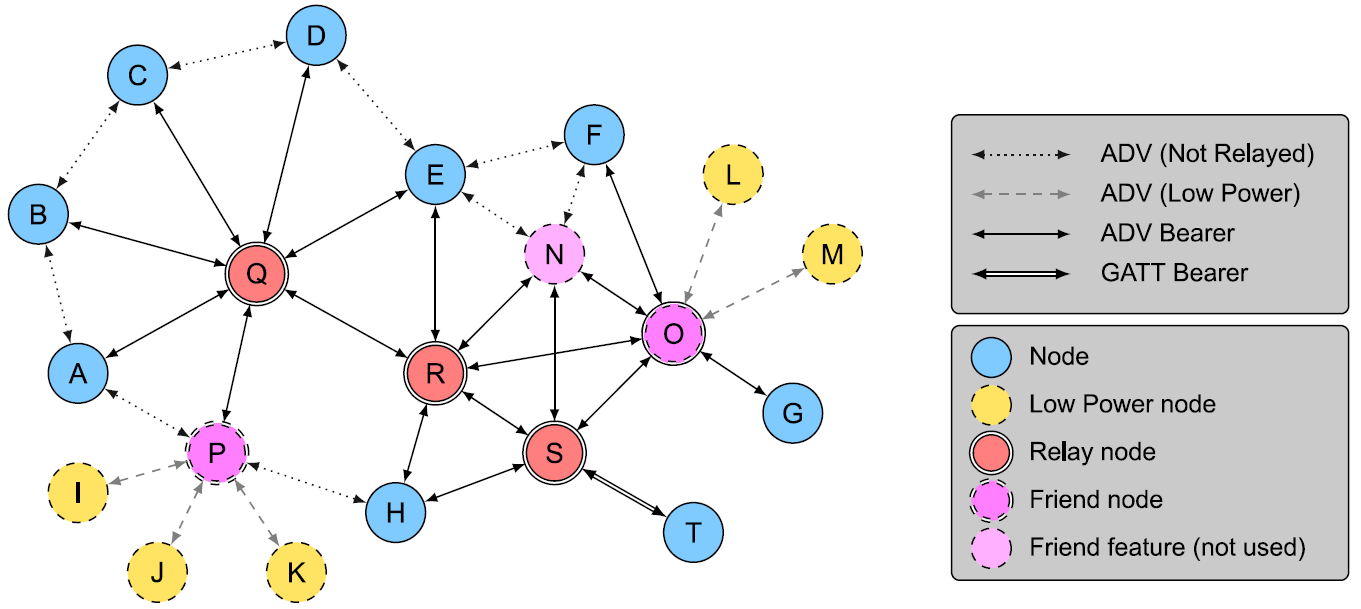
\includegraphics[width=1.0\textwidth]{Bluetooth_Mesh_Topology.PNG}
	\caption{Beispielhafte Topologie eines Bluetooth-Mesh Netzwerks \cite{bluetooth_sig_mesh_netzwerk_spezifikationen_2020}} 
	\label{fig:BTMeshTopology}
\end{figure}


\subsection{Protokoll Stack}\label{sec:BLEMeshProtokollStack}

In diesem Abschnitt wird die Architektur des Mesh-Stacks genauer untersucht. Der Grundsätzliche Aufbau wird Abbildung \ref{fig:BTMeshStack} veranschaulicht. Eine Grafik zur Veranschaulichung des Message-Flows durch die einzelnen Schichten ist im Anhang \ref{app:BluetoothMeshStackLayers} ersichtlich. 

Wie in Kapitel \ref{sec:EinleitungBluetooth} bereits erwähnt basiert der Stack auf Bluetooth Low Energy. Der BLE-Layer dient zur Grundlegenden Schicht des Stacks. Der Zugriff für Mesh-Traffic erfolgt über das GAP-Profil, der für Proxy Traffic über das GATT-Profil. Der Bearer-Layer regelt den Zugriff auf den BLE-Stack. Es existieren verschiedene Bearers. Der GATT-Bearer ermöglicht Geräten ohne GAP Zugriff auf das Netzwerk. Der Advertising-Bearer wird für den Mesh-Traffic benutzt. \\

Der Network-Layer hat folgende Aufgaben zu erfüllen: 

\begin{itemize}
	\item Ver- und Entschlüsselung der Network-PDU
	\item Filtern von nicht relevanten Nachrichten (Adressauflösung)
	\item Relaying von Paketen mittels TTL-Field
\end{itemize}

\begin{wrapfigure}{r}{0.5\textwidth}
	\centering
	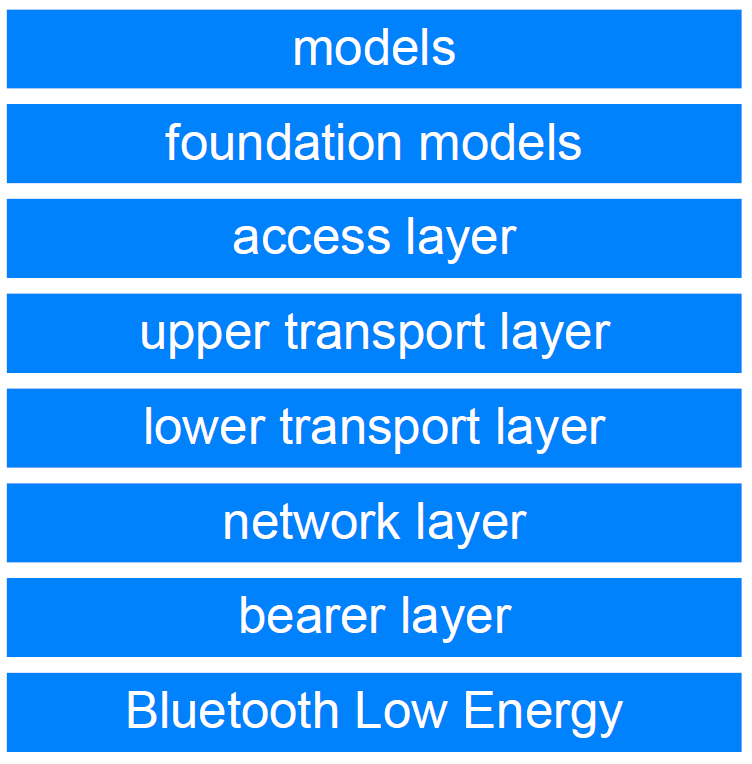
\includegraphics[width=0.5\textwidth]{Bluetooth_Mesh_Stack_Layers.PNG}
	\caption{Bluetooth-Mesh Stack \cite{bluetooth_sig_mesh-technology-overviewpdf_2020}} 
	\label{fig:BTMeshStack}
\end{wrapfigure}

Zudem bedient dieser Layer verschiedene Bearers und ist dafür verantwortlich das alle relevanten Pakete zur entsprechenden Stelle weitergeleitet werden. \\

Über dem Network Layer befindet sich der Transport-Layer, welcher in einen Lower- und Upper-Transport-Layer aufgeteilt ist. Der Lower-Transport-Layer handelt das Acknowledgement einzelner Segmente von eingehenden Nachrichten ab. Zudem beeinhaltet er das Hetz-Stück des Friend-Features, nämlich die Friend-Queue. In diesem Buffer werden alle Nachrichten der  Low-Power-Nodes aufbewahrt. Ebenfalls führt diese Schicht das Segmentieren und Zusammensetzen der Pakete (SAR) durch. Pakete werden in Fragmente aufgeteilt, welche lediglich 8-10 Byte an Applikations-Daten beherbergen können. \\

Der Upper-Transport-Layer dient hauptsächlich zur Ver- und Entschlüsselung von Paketen auf Transport-Ebene. Zudem werden Anfragen wie Friend-Requests über diese Schicht verarbeitet. \\

Der Access-Layer führt die Zuordnung der Nachrichten an die Models durch. Diese Schicht regelt den Zugriff der Applikation auf die unterliegenden Schichten. Zudem werden Nachrichten auf allfällige Replay-Messages geprüft, bevor sie an die Applikation weitergegeben werden. \\

Die zweitletzte Schicht bildet der Foundation-Models-Layer. Seine Aufgabe ist es die Models zu Verwalten, welches über das Config-Server-Model geschieht. Zusätzlich gehört ein Health-Model zu den Foundation-Models, welches den Zustand des Teilnehmers überwacht. Beide Models müssen zwingend auf jedem Node vorhanden sein. \cite{bluetooth_sig_mesh_netzwerk_spezifikationen_2020} \cite{bluetooth_sig_mesh-technology-overviewpdf_2020}  \\

Als letzte Schicht dienen die Models. Dessen Funktionalität ist rein von der Applikation abhängig (siehe Abschnitt \ref{sec:EinleitungBluetooth}). Daher kann diese Schicht als Application-Layer aufgefasst werden.  \\


\subsection{Sicherheit}\label{subsec:BleutoothMeshSicherheit}
Bleutooth-Mesh Nachrichten werden zweifach Verschlüsselt. Die Network-PDU ist mit dem zugehörigen Network-Key gesichert. Wer im Besitz des Netzwerk-Schlüssels gelangt kann Nachrichten bis zum Upper-Transport-Layer auslesen. Für Teilnehmer welche die Nachricht nur weiterleiten (Relayen) müssen reicht dieser Einblick aus. Auf Applikationsebene findet die Verschlüsselung zusätzlich über einen Application-Key statt. Nur Teilnehmer mit dem richtigen Applikation-Key können an Informationen der Models gelangen und diese Steuern. \\

Zusätzlich zur Verschlüsselung führt jeder Teilnehmer eine fortlaufenden Nummerierung der Nachrichten durch (SEQ-Field). Damit lassen sich sogenannte Replay-Attacks verhindern. \\

Um während des Provisioning-Ablauf die Authentifizierung des neuen Teilnehmers sicher zu Stellen, wird ein Device-Key verwendet. Dieser dient einmalig dazu das neue Gerät Einzubinden und zu Konfigurieren. 


\subsection{Grenzen des Stacks}\label{subsec:BLEMeshProtokollStack}

Die Topologie eines Netzwerks beeinträchtigt stark seine Performance. Ist die Node-Dichte sehr hoch, steigt die Wahrscheinlichkeit an das es zu Kollisionen der einzelnen Nachrichten kommt. 

\todo[inline]{Weiter erläutern gemäss ....}

\subsection{Bluetooth Mesh Software Development Kit}\label{sec:BluetoothMeshSoftwareDevelopmentKit}

Die Umsetzung des Bluetooth-Mesh-Stacks ist für die nRF-Platform mittels den folgenden zwei Bibliotheken möglich. 

\begin{itemize}
	\item \textit{\textbf{nRF Connect SDK}}: Auf dem Zephyr-RTOS aufbauende SDK. Zephyr Implementation des Mesh-Stacks, welche von Bluetooth SIG anerkannt ist. Von Nordic nicht zur Verwendung in Endprodukten empfohlen. Unterstützt neuere SOCs wie den nRF5340.  \cite{nordic_semi_welcome_to_the_nrf_connect_sdk_2020}
	\item \textit{\textbf{nRF SDK for Mesh}}: Proprietäre SDK Library von Nordic Semiconductor für Bluetooth-Mesh. Ist zum Einsatz in Endprodukten freigegeben. \cite{nordic_semi_nrf_sdk_for_mesh_2020}
\end{itemize}

Da der neuere SOC nur von der nRF Connect SDK unterstützt wird, sowie die Zephyr Implementation auf weitere SOCs andere Hersteller anwendbar ist, wurde die Implementation mit dieser Bibliothek vorangetrieben. Als Nebenprodukt wurde die Entwicklung mit der nRF SDK for Mesh ins Auge gefasst um die beiden SDKs miteinander zu vergleichen. Zu diesem Zeitpunkt ist ein direkter Vergleich leider noch nicht möglich, da die Funktionalität der nRF SDK for Mesh Variante noch nicht vollständig umgesetzt wurde. 





